\chapter{आयन और आयनिक विलयन}\label{ch:g9:ions}

व्यायामशाला की एक बेंच पर दो स्वच्छ पेय रखे हैं: एक स्पोर्ट्स ड्रिंक की बोतल,
जो अपने ``इलेक्ट्रोलाइटों'' के लिए बिकती है, और चीनी वाले पानी का एक गिलास।
प्रयोगशाला में एक बैटरी और एक छोटे बल्ब से जुड़ी धातु की दो प्लेटें बारी-बारी
से दोनों में डुबोई जाती हैं। स्पोर्ट्स ड्रिंक में बल्ब जल उठता है; चीनी वाले
पानी में वह बुझा रहता है। पहले द्रव में कुछ ऐसा है जो विद्युत आवेश ढोता है,
और चीनी ऐसा नहीं करती। वह कुछ है --- \omterm{def:g9:ions:ion}{आयन}।

\begin{recall}
\omterm{def:g7:atoms-and-molecules:atom}{परमाणु} के \omterm{def:g9:inside-the-atom:nucleus}{नाभिक} में $Z$ \omterm{def:g9:inside-the-atom:proton}{प्रोटॉन} होते हैं, हर एक पर आवेश $+e$, और उसके चारों
ओर $Z$ \omterm{def:g9:inside-the-atom:nucleus}{इलेक्ट्रॉन}, हर एक पर आवेश $-e$: \omterm{def:g7:atoms-and-molecules:atom}{परमाणु} उदासीन होता है
(\cref{ch:g9:inside-the-atom})। पानी में घुला \omterm{def:g6:solutions-and-solubility:solute}{विलेय} एक
\omterm{def:g6:solutions-and-solubility:solute}{जलीय विलयन} देता है (\cref{ch:g6:solutions-and-solubility})। \omterm{def:g7:identifying-substances:characteristic-test}{अभिलाक्षणिक
परीक्षण} किसी स्पीशीज़ को एक दिखाई देने वाले परिणाम से पहचानता है
(\cref{ch:g7:identifying-substances})।
\end{recall}

\begin{omfigure}
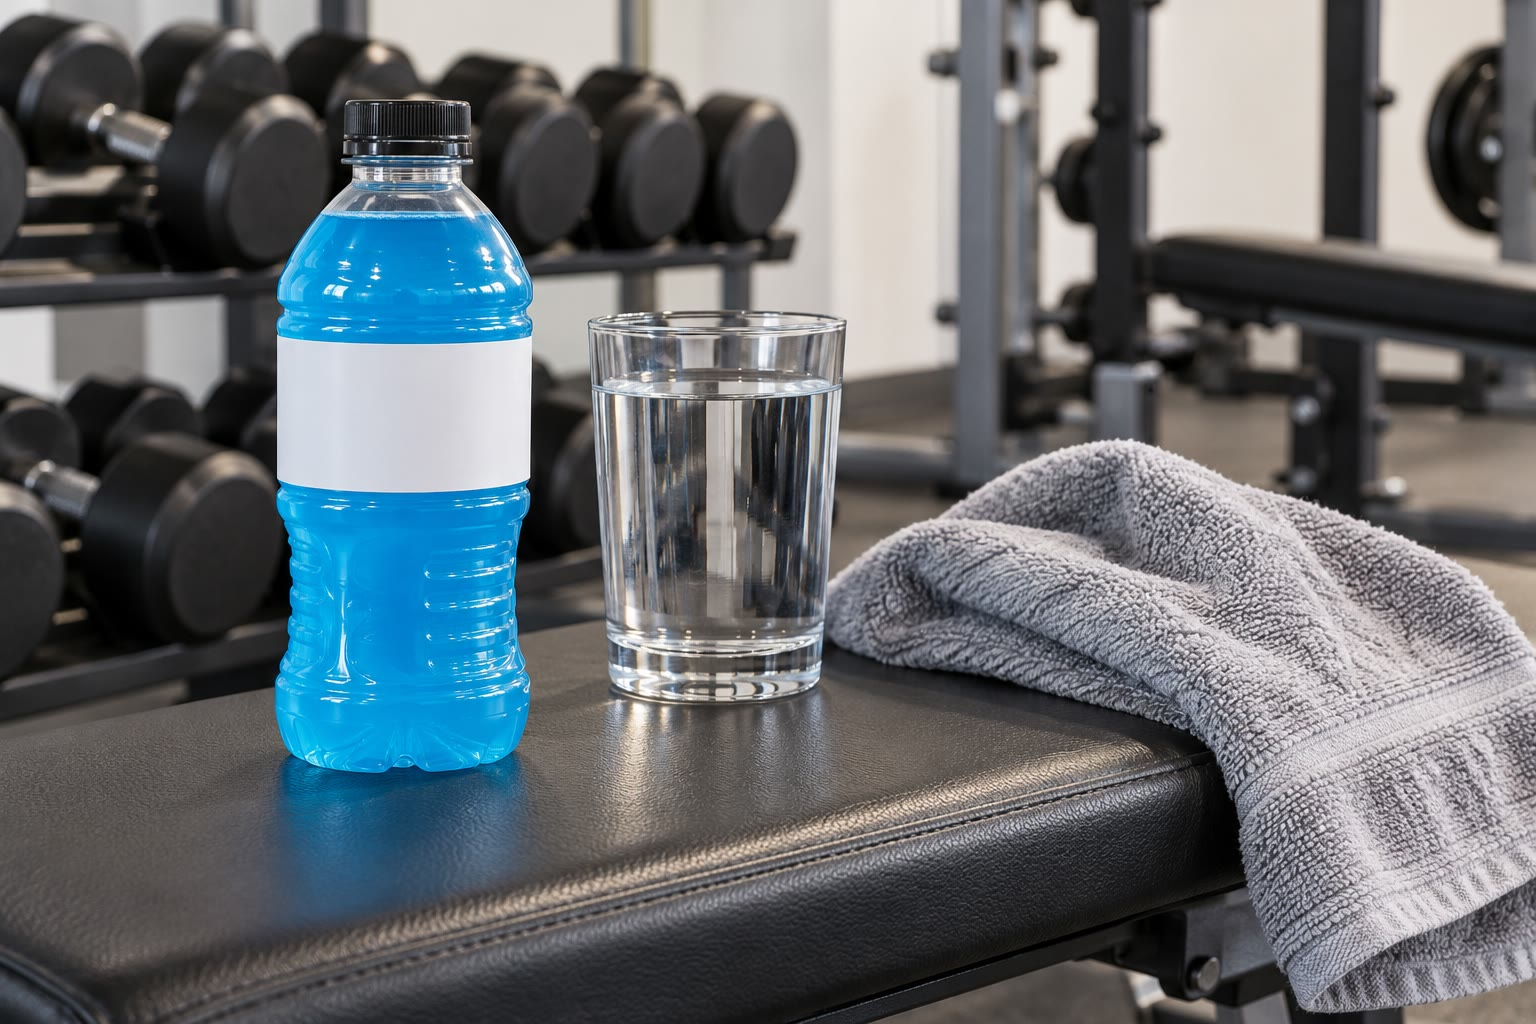
\includegraphics[width=0.5\linewidth]{images/book1/ai/g9-sports-drink.jpg}

{\small एक स्पोर्ट्स ड्रिंक और पानी का एक गिलास: पेय में घुले हुए
\omterm{def:g9:ions:ion}{आयन} हैं।}
\end{omfigure}

\section{इलेक्ट्रॉन लेने या खोने वाले परमाणु}

\begin{definition}[आयन, धनायन, ऋणायन]\label{def:g9:ions:ion}
\emph{आयन}\index{आयन} ऐसा \omterm{def:g7:atoms-and-molecules:atom}{परमाणु}, या \omterm{def:g7:atoms-and-molecules:atom}{परमाणुओं} का ऐसा समूह, है जिसने एक या
अधिक \omterm{def:g9:inside-the-atom:nucleus}{इलेक्ट्रॉन} खोए या लिए हैं, और इसलिए जिस पर विद्युत आवेश है। \omterm{def:g9:inside-the-atom:nucleus}{इलेक्ट्रॉन}
खोकर धनात्मक आवेश वाला आयन
\emph{धनायन}\index{धनायन} है; \omterm{def:g9:inside-the-atom:nucleus}{इलेक्ट्रॉन} लेकर ऋणात्मक आवेश वाला आयन
\emph{ऋणायन}\index{ऋणायन} है। आवेश सूत्र के दाईं ओर ऊपर
लिखा जाता है: \ce{Na+}, \ce{Cu^{2+}}, \ce{Cl-}।
\end{definition}

\begin{example}[सोडियम और क्लोरीन]\label{ex:g9:ions:na-cl}
सोडियम \omterm{def:g7:atoms-and-molecules:atom}{परमाणु}, 11 \omterm{def:g9:inside-the-atom:proton}{प्रोटॉन} और 11 \omterm{def:g9:inside-the-atom:nucleus}{इलेक्ट्रॉन}, एक \omterm{def:g9:inside-the-atom:nucleus}{इलेक्ट्रॉन} खोता है: वह
सोडियम \omterm{def:g9:ions:ion}{आयन} \ce{Na+} बन जाता है, 11 \omterm{def:g9:inside-the-atom:proton}{प्रोटॉन} और 10 \omterm{def:g9:inside-the-atom:nucleus}{इलेक्ट्रॉन}, आवेश
$+1$:
\[
  \ce{Na -> Na+ + e-}.
\]
क्लोरीन \omterm{def:g7:atoms-and-molecules:atom}{परमाणु}, 17 \omterm{def:g9:inside-the-atom:proton}{प्रोटॉन} और 17 \omterm{def:g9:inside-the-atom:nucleus}{इलेक्ट्रॉन}, एक \omterm{def:g9:inside-the-atom:nucleus}{इलेक्ट्रॉन} लेता है: वह
क्लोराइड \omterm{def:g9:ions:ion}{आयन} \ce{Cl-} बन जाता है, 17 \omterm{def:g9:inside-the-atom:proton}{प्रोटॉन} और 18 \omterm{def:g9:inside-the-atom:nucleus}{इलेक्ट्रॉन}:
\[
  \ce{Cl + e- -> Cl-}.
\]
\end{example}

\begin{omfigure}
\begin{tikzpicture}[font=\small]
  \foreach \x/\name/\p/\e/\ch/\col in {0/{सोडियम परमाणु}/11/11/0/omDef,
      3.7/{सोडियम आयन \ce{Na+}}/11/10/+1/omProp,
      8.0/{क्लोरीन परमाणु}/17/17/0/omDef, 11.7/{क्लोराइड आयन \ce{Cl-}}/17/18/$-1$/omProp} {
    \node[draw=\col, fill=\col!6, rounded corners=2pt, align=center, text width=2.4cm]
      at (\x,0) {\textbf{\name}\\ \p\ प्रोटॉन\\ \e\ इलेक्ट्रॉन\\ आवेश \ch};
  }
  \draw[->, thick, omProp] (1.45,0) -- (2.25,0) node[midway, above, text=black,
    font=\footnotesize, align=center] {खोता है\\ 1 \ce{e-}};
  \draw[->, thick, omProp] (9.45,0) -- (10.25,0) node[midway, above, text=black,
    font=\footnotesize, align=center] {लेता है\\ 1 \ce{e-}};
\end{tikzpicture}

{\small सोडियम \omterm{def:g7:atoms-and-molecules:atom}{परमाणु} एक \omterm{def:g9:inside-the-atom:nucleus}{इलेक्ट्रॉन} खोकर सोडियम \omterm{def:g9:ions:ion}{आयन} बनता है; क्लोरीन
\omterm{def:g7:atoms-and-molecules:atom}{परमाणु} एक \omterm{def:g9:inside-the-atom:nucleus}{इलेक्ट्रॉन} लेकर क्लोराइड \omterm{def:g9:ions:ion}{आयन} बनता है। \omterm{def:g9:inside-the-atom:proton}{प्रोटॉन} नहीं
बदलते।}
\end{omfigure}

\begin{proposition}[कुछ आम आयन]\label{prop:g9:ions:common}
एकपरमाणुक \omterm{def:g9:ions:ion}{आयन} एक \omterm{def:g7:atoms-and-molecules:atom}{परमाणु} से बनते हैं; बहुपरमाणुक \omterm{def:g9:ions:ion}{आयन} \omterm{def:g7:atoms-and-molecules:atom}{परमाणुओं} के ऐसे समूह से
जो साथ बना रहता है:
\begin{center}
\small
\begin{tabular}{llll}
\hline
\omterm{def:g9:ions:ion}{धनायन} & & \omterm{def:g9:ions:ion}{ऋणायन} & \\
\hline
सोडियम & \ce{Na+} & क्लोराइड & \ce{Cl-} \\
पोटैशियम & \ce{K+} & हाइड्रॉक्साइड & \ce{OH-} \\
कैल्सियम & \ce{Ca^{2+}} & नाइट्रेट & \ce{NO3-} \\
मैग्नीशियम & \ce{Mg^{2+}} & कार्बोनेट & \ce{CO3^{2-}} \\
कॉपर(II) & \ce{Cu^{2+}} & सल्फ़ेट & \ce{SO4^{2-}} \\
आयरन(II), आयरन(III) & \ce{Fe^{2+}}, \ce{Fe^{3+}} & & \\
ज़िंक & \ce{Zn^{2+}} & & \\
ऐलुमिनियम & \ce{Al^{3+}} & & \\
अमोनियम & \ce{NH4+} & & \\
\hline
\end{tabular}
\end{center}
\end{proposition}

\section{आयनिक यौगिक और उनके सूत्र}

\begin{definition}[आयनिक यौगिक]\label{def:g9:ions:ionic-compound}
\emph{आयनिक यौगिक}\index{आयनिक यौगिक} \omterm{def:g9:ions:ion}{धनायनों} और \omterm{def:g9:ions:ion}{ऋणायनों} से ऐसी संख्याओं
में बना होता है कि पूरे पर कोई आवेश न हो। उसका सूत्र \omterm{def:g9:ions:ion}{आयनों} का अनुपात
बताता है, उनके आवेशों के बिना: सोडियम क्लोराइड के लिए \ce{NaCl},
एक \ce{Na+} पर एक \ce{Cl-}; कैल्सियम क्लोराइड के लिए \ce{CaCl2},
दो \ce{Cl-} पर एक \ce{Ca^{2+}}।
\end{definition}

\begin{method}[आयनिक यौगिक का सूत्र लिखना]\label{met:g9:ions:formula}
\begin{enumerate}
  \item दोनों \omterm{def:g9:ions:ion}{आयनों} को उनके आवेशों के साथ लिखो, पहले \omterm{def:g9:ions:ion}{धनायन}।
  \item हर एक की वे सबसे छोटी संख्याएँ खोजो जिनसे कुल आवेश
        शून्य हो जाए।
  \item इन संख्याओं को \omterm{def:g7:atoms-and-molecules:formula}{पादांकों} के रूप में लिखो; जिस बहुपरमाणुक \omterm{def:g9:ions:ion}{आयन} को
        \omterm{def:g7:atoms-and-molecules:formula}{पादांक} चाहिए, वह कोष्ठक में जाता है।
\end{enumerate}
ऐलुमिनियम ऑक्साइड: \ce{Al^{3+}} और \ce{O^{2-}}; $2 \times (+3) + 3 \times
(-2) = 0$, इसलिए \ce{Al2O3}। आयरन(III) हाइड्रॉक्साइड: \ce{Fe^{3+}} और तीन
\ce{OH-}: \ce{Fe(OH)3}।
\end{method}

\begin{proposition}[आयनिक ठोस आयनों का ढेर है]\label{prop:g9:ions:solid}
नमक के क्रिस्टल में सोडियम \omterm{def:g9:ions:ion}{आयन} और क्लोराइड \omterm{def:g9:ions:ion}{आयन} एक नियमित त्रिविमीय ढेर में
बारी-बारी से आते हैं, और हर \omterm{def:g9:ions:ion}{आयन} विपरीत आवेश वाले \omterm{def:g9:ions:ion}{आयनों} से घिरा होता है, जो
उसे अपनी जगह थामे रखते हैं। खाने के नमक के एक दाने में अरबों-खरबों \omterm{def:g9:ions:ion}{आयन} होते
हैं; उसकी घनाकार आकृति घनाकार ढेर को दर्शाती है।
\end{proposition}

\begin{omfigure}
\begin{minipage}[b]{0.5\linewidth}\centering
\begin{tikzpicture}[font=\small]
  \foreach \i in {0,...,5} \foreach \j in {0,...,4} {
    \pgfmathtruncatemacro\pp{mod(\i+\j,2)}
    \ifnum\pp=0 \node[aNa, minimum size=5mm] at (0.62*\i,0.62*\j) {};
    \else \node[aCl, minimum size=7.4mm] at (0.62*\i,0.62*\j) {};\fi
  }
\end{tikzpicture}

{\small नमक के क्रिस्टल की एक परत: सोडियम \omterm{def:g9:ions:ion}{आयन} (बैंगनी, छोटे) और
क्लोराइड \omterm{def:g9:ions:ion}{आयन} (हरे) बारी-बारी से आते हैं।}
\end{minipage}\hfill
\begin{minipage}[b]{0.3\linewidth}\centering
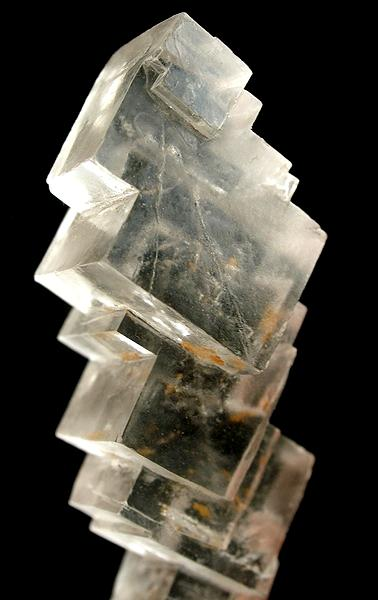
\includegraphics[height=4.6cm]{images/book1/halite.jpg}

{\small हैलाइट, प्राकृतिक सेंधा नमक। फ़ोटो: रॉबर्ट एम.~लेविंस्की,
CC BY-SA 3.0।}
\end{minipage}
\end{omfigure}

\section{आयनिक विलयन विद्युत का चालन करते हैं}

\begin{notation}[अवस्था-संकेत (aq)]\label{not:g9:ions:aq}
पानी में घुले \omterm{def:g9:ions:ion}{आयन} या \omterm{def:g7:atoms-and-molecules:molecule}{अणु} पर (aq) लगाया जाता है, यानी जलीय:
\ce{Na+(aq)}, \ce{Cl-(aq)}।
\end{notation}

\begin{proposition}[आयनिक विलयन विद्युत का चालन करते हैं]\label{prop:g9:ions:conduct}
जब कोई \omterm{def:g9:ions:ionic-compound}{आयनिक यौगिक} पानी में \omterm{def:g2:mixing-and-dissolving:dissolve}{घुलता} है, तो उसके \omterm{def:g9:ions:ion}{आयन} अलग हो जाते हैं और विलयन
में स्वतंत्र रूप से घूमते हैं: नमकीन पानी में \ce{Na+(aq)} और
\ce{Cl-(aq)} होते हैं। गतिशील \omterm{def:g9:ions:ion}{आयन} विद्युत आवेश ढोते हैं, इसलिए आयनिक विलयन
विद्युत का चालन करता है। चीनी का विलयन, जिसके \omterm{def:g7:atoms-and-molecules:molecule}{अणुओं} पर कोई आवेश नहीं होता,
चालन नहीं करता; बहुत शुद्ध पानी भी नहीं।
\end{proposition}

\begin{inthelab}[कौन-से द्रव चालन करते हैं?]
शिक्षक धातु की दो प्लेटों, कम वोल्टता की एक बैटरी और एक छोटे बल्ब को एक
परिपथ में जोड़ते हैं; प्लेटें बारी-बारी से आसुत जल, चीनी के पानी, नमकीन पानी
और कॉपर सल्फ़ेट के विलयन में डुबोई जाती हैं, और हर बार के बीच धोई जाती हैं।
बल्ब केवल दोनों आयनिक विलयनों के साथ जलता है।
\end{inthelab}

\begin{omfigure}
\begin{tikzpicture}[font=\small, scale=1.1]
  \foreach \xs/\lit/\lab in {0/1/{नमकीन पानी: बल्ब जलता है}, 5.2/0/{चीनी का पानी: बल्ब बुझा रहता है}} {
    \begin{scope}[xshift=\xs cm]
      \pic[transform shape] at (2,0) {beaker={0.7}{omWater!80}};
      \fill[black!45] (1.6,0.25) rectangle (1.7,2.6);
      \fill[black!45] (2.3,0.25) rectangle (2.4,2.6);
      \ifnum\lit=1 \fill[yellow!70, opacity=0.8] (3.4,3.0) circle (0.42);\fi
      \draw (1.65,2.6) -- (1.65,3.6) to[battery1] (3.4,3.6) -- (3.4,3.4)
        to[lamp] (3.4,2.6) -- (2.35,2.6);
      \node[anchor=north, align=center] at (2,-0.15) {\lab};
    \end{scope}
  }
\end{tikzpicture}

{\small चालकता परीक्षण: नमकीन पानी के साथ \omterm{def:g9:ions:ion}{आयन} धारा ढोते हैं और बल्ब जलता
है; चीनी के पानी में कोई \omterm{def:g9:ions:ion}{आयन} नहीं होते और बल्ब बुझा
रहता है।}
\end{omfigure}

\section{आयनों के लिए अवक्षेपण परीक्षण}

\begin{definition}[अवक्षेप]\label{def:g9:ions:precipitate}
जब दो विलयन मिलाए जाते हैं, तो एक का \omterm{def:g9:ions:ion}{धनायन} और दूसरे का \omterm{def:g9:ions:ion}{ऋणायन} ऐसा \omterm{def:g9:ions:ionic-compound}{आयनिक
यौगिक} बना सकते हैं जो \omterm{def:g2:mixing-and-dissolving:dissolve}{घुलता} नहीं। वह एक बारीक ठोस के रूप में प्रकट होता है जो
द्रव को धुँधला कर देता है और नीचे बैठ जाता है: यह
\emph{अवक्षेप}\index{अवक्षेप} है। यह अभिक्रिया
\emph{अवक्षेपण}\index{अवक्षेपण} कहलाती है।
\end{definition}

\begin{proposition}[आम आयनों के परीक्षण]\label{prop:g9:ions:tests}
किसी \omterm{def:g7:identifying-substances:characteristic-test}{अभिकर्मक} विलयन की कुछ बूँदें किसी \omterm{def:g9:ions:ion}{आयन} को उससे बनने वाले \omterm{def:g9:ions:precipitate}{अवक्षेप} के
रंग से पहचान लेती हैं:
\begin{center}
\small
\begin{tabular}{llll}
\hline
खोजा जाने वाला \omterm{def:g9:ions:ion}{आयन} & \omterm{def:g7:identifying-substances:characteristic-test}{अभिकर्मक} & \omterm{def:g9:ions:precipitate}{अवक्षेप} & रंग \\
\hline
कॉपर(II) \ce{Cu^{2+}} & सोडियम हाइड्रॉक्साइड & \ce{Cu(OH)2} & नीला \\
आयरन(II) \ce{Fe^{2+}} & सोडियम हाइड्रॉक्साइड & \ce{Fe(OH)2} & हरा \\
आयरन(III) \ce{Fe^{3+}} & सोडियम हाइड्रॉक्साइड & \ce{Fe(OH)3} & नारंगी-भूरा \\
ज़िंक \ce{Zn^{2+}} & सोडियम हाइड्रॉक्साइड & \ce{Zn(OH)2} & सफ़ेद \\
ऐलुमिनियम \ce{Al^{3+}} & सोडियम हाइड्रॉक्साइड & \ce{Al(OH)3} & सफ़ेद \\
क्लोराइड \ce{Cl-} & सिल्वर नाइट्रेट & \ce{AgCl} & सफ़ेद, प्रकाश में काला पड़ता है \\
\hline
\end{tabular}
\end{center}
\end{proposition}

\begin{example}[अवक्षेपण लिखना]\label{ex:g9:ions:equation}
केवल वे \omterm{def:g9:ions:ion}{आयन} लिखे जाते हैं जो ठोस बनाते हैं; बाकी घुले रहते हैं
और भाग नहीं लेते:
\[
  \ce{Cu^{2+}(aq) + 2OH-(aq) -> Cu(OH)2(s)}, \qquad
  \ce{Ag+(aq) + Cl-(aq) -> AgCl(s)}.
\]
\end{example}

\begin{omfigure}
\begin{tikzpicture}[font=\small, scale=0.95]
  \foreach \k/\pc/\lab in {0/blue!60/{\ce{Cu^{2+}}: नीला}, 1/green!45!black!70/{\ce{Fe^{2+}}: हरा},
      2/orange!70!brown/{\ce{Fe^{3+}}: नारंगी-\\भूरा}, 3/white!85!black/{\ce{Zn^{2+}}: सफ़ेद},
      4/white!85!black/{\ce{Al^{3+}}: सफ़ेद}, 5/white!80!black/{\ce{Cl-}: सफ़ेद}} {
    \pic[transform shape] at (\k*2.3,0) {testtube={0.5}{omWater!60}};
    \pic[transform shape] at (\k*2.3,0) {testtube={0.14}{\pc}};
    \node[anchor=north, align=center, font=\footnotesize, text width=2cm] at (\k*2.3,-0.15) {\lab};
  }
\end{tikzpicture}

{\small सोडियम हाइड्रॉक्साइड के साथ बने \omterm{def:g9:ions:precipitate}{अवक्षेप} (पहली पाँच नलियाँ) और
सिल्वर नाइट्रेट के साथ (आख़िरी नली)।}
\end{omfigure}

\begin{safety}{\ghs[0.82cm]{GHS05}\ghs[0.82cm]{GHS07}}
% ledger: ghs:NaOH, ghs:AgNO3
सोडियम हाइड्रॉक्साइड: त्वचा को गंभीर रूप से जलाता है और आँखों को हानि पहुँचाता
है, और धातुओं के लिए संक्षारक हो सकता है (GHS05); तनु रूप में त्वचा और आँखों में
जलन करता है (GHS07)। सिल्वर नाइट्रेट, क्लोराइड का
\omterm{def:g7:identifying-substances:characteristic-test}{अभिकर्मक}, एक ऑक्सीकारक है, संक्षारक है और जलीय जीवों के लिए अत्यंत विषैला है।
चश्मा, दस्ताने; \omterm{def:g7:identifying-substances:characteristic-test}{अभिकर्मक} शिक्षक बूँद-बूँद करके देते हैं।
\end{safety}

\begin{method}[किसी आयन का परीक्षण]\label{met:g9:ions:test}
\begin{enumerate}
  \item परखे जाने वाले विलयन की थोड़ी मात्रा एक परखनली में डालो।
  \item \omterm{def:g7:identifying-substances:characteristic-test}{अभिकर्मक} बूँद-बूँद करके मिलाओ।
  \item बने हुए किसी भी \omterm{def:g9:ions:precipitate}{अवक्षेप} का रंग नोट करो और सारणी से तुलना करो।
  \item निष्कर्ष निकालो, और याद रखो कि परीक्षण किसी \omterm{def:g9:ions:ion}{आयन} को पहचानता है, यौगिक
        को नहीं: आयरन(III) क्लोराइड का विलयन
        \ce{Fe^{3+}} परीक्षण और \ce{Cl-} परीक्षण दोनों देता है।
\end{enumerate}
\end{method}

\section{अभ्यास}

\begin{exercise}[$\star$]\label{exo:g9:ions:1}
\omterm{def:g9:ions:ion}{आयन} क्या है? \omterm{def:g9:ions:ion}{धनायन} और \omterm{def:g9:ions:ion}{ऋणायन} में क्या अंतर है?
\end{exercise}

\begin{exercise}[$\star$]\label{exo:g9:ions:2}
एक मैग्नीशियम \omterm{def:g7:atoms-and-molecules:atom}{परमाणु} (12 \omterm{def:g9:inside-the-atom:proton}{प्रोटॉन}) दो \omterm{def:g9:inside-the-atom:nucleus}{इलेक्ट्रॉन} खोता है। बने हुए \omterm{def:g9:ions:ion}{आयन} का सूत्र
लिखो, और उसके \omterm{def:g9:inside-the-atom:proton}{प्रोटॉनों} और \omterm{def:g9:inside-the-atom:nucleus}{इलेक्ट्रॉनों} की संख्या बताओ।
\end{exercise}

\begin{exercise}[$\star$]\label{exo:g9:ions:3}
पोटैशियम क्लोराइड, मैग्नीशियम क्लोराइड और कैल्सियम ऑक्साइड के सूत्र लिखो
(ऑक्साइड \omterm{def:g9:ions:ion}{आयन}: \ce{O^{2-}})।
\end{exercise}

\begin{exercise}[$\star$]\label{exo:g9:ions:4}
नमकीन पानी विद्युत का चालन क्यों करता है, जबकि चीनी का पानी नहीं?
\end{exercise}

\begin{exercise}[$\star\star$]\label{exo:g9:ions:5}
कॉपर(II) सल्फ़ेट, ऐलुमिनियम क्लोराइड और सोडियम
कार्बोनेट के सूत्र लिखो।
\end{exercise}

\begin{exercise}[$\star\star$]\label{exo:g9:ions:6}
किसी विलयन में सोडियम हाइड्रॉक्साइड मिलाने पर नारंगी-भूरा \omterm{def:g9:ions:precipitate}{अवक्षेप} बनता है।
विलयन में कौन-सा \omterm{def:g9:ions:ion}{आयन} है? \omterm{def:g9:ions:precipitate}{अवक्षेपण} का
समीकरण लिखो।
\end{exercise}

\begin{exercise}[$\star\star$]\label{exo:g9:ions:7}
सल्फ़ेट \omterm{def:g9:ions:ion}{आयन} \ce{SO4^{2-}} पर उसके \omterm{def:g9:inside-the-atom:proton}{प्रोटॉनों} से कितने \omterm{def:g9:inside-the-atom:nucleus}{इलेक्ट्रॉन} अधिक
हैं? नाइट्रेट \omterm{def:g9:ions:ion}{आयन} \ce{NO3-} पर?
\end{exercise}

\begin{exercise}[$\star\star$]\label{exo:g9:ions:8}
एक विलयन सिल्वर नाइट्रेट के साथ सफ़ेद \omterm{def:g9:ions:precipitate}{अवक्षेप} और सोडियम हाइड्रॉक्साइड के साथ
नीला \omterm{def:g9:ions:precipitate}{अवक्षेप} देता है। घुले हुए \omterm{def:g9:ions:ionic-compound}{आयनिक यौगिक} का नाम बताओ और उसका
सूत्र लिखो।
\end{exercise}

\begin{exercise}[$\star\star$]\label{exo:g9:ions:9}
नमक के क्रिस्टल की परत वाला चित्र देखो। परत के बीच के किसी \omterm{def:g9:ions:ion}{आयन} के इस परत में
विपरीत आवेश वाले कितने पड़ोसी हैं?
\end{exercise}

\begin{exercise}[$\star\star$]\label{exo:g9:ions:10}
\ce{Fe^{2+}} और \ce{OH-} \omterm{def:g9:ions:ion}{आयनों} से आयरन(II) हाइड्रॉक्साइड के
\omterm{def:g9:ions:precipitate}{अवक्षेपण} का समीकरण लिखो।
\end{exercise}

\begin{exercise}[$\star\star\star$]\label{exo:g9:ions:11}
एक सफ़ेद चूर्ण ज़िंक क्लोराइड या सोडियम क्लोराइड हो सकता है। पानी में घोलने
पर वह सोडियम हाइड्रॉक्साइड के साथ सफ़ेद \omterm{def:g9:ions:precipitate}{अवक्षेप} देता है। वह कौन-सा है?
समीकरण लिखो।
\end{exercise}

\begin{exercise}[$\star\star\star$]\label{exo:g9:ions:12}
कैल्सियम क्लोराइड के क्रिस्टल में कैल्सियम के 1000 \omterm{def:g9:ions:ion}{आयनों} पर कितने क्लोराइड
\omterm{def:g9:ions:ion}{आयन} हैं? जाँचो कि क्रिस्टल उदासीन है।
\end{exercise}

\section{समस्या: जंग वाला कुआँ}

\begin{problem}[{सप्ताहांत समस्या --- एक फ़ार्महाउस के सिंक में नारंगी दाग़,
दो परीक्षण, और कुएँ के एक लीटर पानी में लोहे के आयनों की संख्या}]
\label{pb:g9:ions:1}
एक फ़ार्महाउस के कुएँ का पानी सिंक में नारंगी दाग़ छोड़ता है। एक प्रयोगशाला को
उसका नमूना मिलता है। ताज़ा निकाला गया पानी स्वच्छ है; सोडियम हाइड्रॉक्साइड के
साथ वह हरा \omterm{def:g9:ions:precipitate}{अवक्षेप} देता है, जो एक घंटे के भीतर सतह पर, जहाँ वह \omterm{def:g4:air-a-mixture-of-gases:air}{वायु} के संपर्क में
आता है, नारंगी-भूरा हो जाता है। प्रयोगशाला प्रति लीटर \qty{0.30}{mg} लोहा
मापती है, जो लोहे के \omterm{def:g9:ions:ion}{आयनों} के रूप में है। एक \omterm{def:g9:inside-the-atom:proton}{न्यूक्लिऑन} का द्रव्यमान
\qty{1.67e-27}{kg} लो, और लोहे के एक \omterm{def:g7:atoms-and-molecules:atom}{परमाणु} के लिए 56
\omterm{def:g9:inside-the-atom:proton}{न्यूक्लिऑन}।

\medskip
\noindent\textbf{भाग I --- परीक्षण।}
\begin{enumerate}
  \item हरा \omterm{def:g9:ions:precipitate}{अवक्षेप} कौन-सा \omterm{def:g9:ions:ion}{आयन} दिखाता है? \omterm{def:g9:ions:precipitate}{अवक्षेप} का सूत्र
        बताओ।
  \item नारंगी-भूरा \omterm{def:g9:ions:precipitate}{अवक्षेप} कौन-सा \omterm{def:g9:ions:ion}{आयन} दिखाता है? उसका
        सूत्र बताओ।
  \item आयरन(II) \omterm{def:g9:ions:ion}{आयन} और आयरन(III) \omterm{def:g9:ions:ion}{आयन} में एक \omterm{def:g9:inside-the-atom:nucleus}{इलेक्ट्रॉन} का अंतर है।
        किसमें ज़्यादा \omterm{def:g9:inside-the-atom:nucleus}{इलेक्ट्रॉन} हैं? हर एक में कितने \omterm{def:g9:inside-the-atom:nucleus}{इलेक्ट्रॉन} हैं
        (लोहा: $Z = 26$)?
  \item आयरन(III) हाइड्रॉक्साइड के \omterm{def:g9:ions:precipitate}{अवक्षेपण} का समीकरण लिखो।
\end{enumerate}

\medskip
\noindent\textbf{भाग II --- दाग़।}
\begin{enumerate}[resume]
  \item सिंक में स्वच्छ पानी धीरे-धीरे धुँधला और नारंगी हो जाता है। कुएँ से
        निकलते समय पानी में कौन-सा \omterm{def:g9:ions:ion}{आयन} होता है, और अंत में उसमें कौन-सा
        \omterm{def:g9:ions:ion}{आयन} रह जाता है?
  \item आयरन(III) \omterm{def:g9:ions:ion}{आयनों} और हाइड्रॉक्साइड \omterm{def:g9:ions:ion}{आयनों} से बने \omterm{def:g9:ions:ionic-compound}{आयनिक यौगिक} का सूत्र
        लिखो, और जाँचो कि वह उदासीन है।
  \item क्या कुएँ से निकलते ही पानी को छानकर उसका लोहा हटाया जा सकता है?
        नारंगी हो जाने के बाद? समझाओ।
  \item क्या लोहे के \omterm{def:g9:ions:ion}{आयनों} वाला पानी \omterm{def:g6:pure-substances-and-mixtures:pure-substance}{शुद्ध पदार्थ} है? \omterm{def:g6:pure-substances-and-mixtures:homogeneous}{समांगी
        मिश्रण}?
\end{enumerate}

\medskip
\noindent\textbf{भाग III --- \omterm{def:g9:ions:ion}{आयनों} की गिनती।}
\begin{enumerate}[resume]
  \item लोहे के एक \omterm{def:g7:atoms-and-molecules:atom}{परमाणु} का द्रव्यमान किलोग्राम में निकालो।
  \item \qty{0.30}{mg} को किलोग्राम में बदलो।
  \item लोहे के \omterm{def:g9:ions:ion}{आयन} का द्रव्यमान लोहे के \omterm{def:g7:atoms-and-molecules:atom}{परमाणु} के द्रव्यमान के बराबर क्यों
        माना जा सकता है?
  \item कुएँ के पानी के एक लीटर में लोहे के \omterm{def:g9:ions:ion}{आयनों} की संख्या निकालो।
\end{enumerate}
\end{problem}
